\chapter{Modelos Te\'{o}ricos}
<<<<<<< HEAD
La din\'{a}mica de una biomol\'{e}cula se determina por las ecuaciones de movimiento para cada uno de los \'{a}tomos que la constituyen. Usualmente en una biomol\'{e}cula el n\'{u}mero de mon\'{o}meros es mayor a 20, que al multiplicarlo por el n\'{u}mero de \'{a}tomos en cada mon\'{o}mero incrementa considerablemente el n\'{u}mero de ecuaciones de movimiento a resolver, de ah\'{i} que sea necesario realizar \textit{din\'{a}mica molecular} (Molecular Dynamics por sus siglas en ingl\'{e}s MD) la cual estudia mediante simulaciones computacionales el movimiento de los \'{a}tomos de acuerdo a las interacciones que presenten.\\
=======
La din\'{a}mica de una biomol\'{e}cula se determina por las ecuaciones de movimiento para cada uno de los \'{a}tomos que la constituyen. Usualmente en una biomol\'{e}cula el n\'{u}mero de mon\'{o}meros es mayor a 20, que al multiplicarlo por el n\'{u}mero de \'{a}tomos en cada mon\'{o}mero incrementa considerablemente el n\'{u}mero de ecuaciones de movimiento a resolver, de ah\'{i} que sea necesario realizar \textit{din\'{a}mica molecular} (Molecular Dynamics que por sus siglas en ingl\'{e}s es MD) la cual estudia mediante simulaciones computacionales el movimiento de los \'{a}tomos, de acuerdo a las interacciones que presenten.\\
>>>>>>> b7135250bc9138189c3783a0d80fda1228288f7e

Las ecuaciones de movimiento se pueden conocer a partir de los formalismos lagrangiano o hamiltoniano \cite{Goldstein2001ClassicalMechanics}, en los cuales es necesario conocer los potenciales con los que interact\'{u}an los \'{a}tomos. Las soluciones a las ecuaciones de movimiento se encuentran mediante los m\'{e}todos de la din\'{a}mica molecular o los an\'{a}lisis de modos normales (Normal Mode Analysis que por sus siglas en ingl\'{e}s es NMA) en los cuales se escogen los modelos de potencial.\\

Los diversos modelos de potencial pueden ser tomados seg\'{u}n la naturaleza del pol\'{i}mero a analizar, ver \cite{Lezon2009ElasticViruses}. Sin embargo, al escoger el potencial  para hacer un an\'{a}lisis \textit{in silico} de la din\'{a}mica de una biomol\'{e}cula, debe tenerse en cuenta el costo computacional requerido, esto es, el tiempo de simulaci\'{o}n de la mol\'{e}cula y la exactitud requerida en el movimiento de cada uno de los constituyentes de la mol\'{e}cula.\\

De acuerdo a los par\'{a}metros de costo y tiempo, las simulaciones de biomol\'{e}culas se pueden hacer analizando los \textit{movimientos locales} y los \textit{movimientos globales}.

\section{Movimientos Globales}

Son aqu\'{e}llas simulaciones en las que se desean conocer los \textit{cambios globales} o el aspecto general que excibe el movimiento de una biomol\'{e}cula haciendo simplificaciones, ya sea en los potenciales presentes en la biomol\'{e}cula como en el n\'{u}mero de \'{a}tomos interconectados. Este tipo de simulaciones pueden ser realizadas a un orden de magnitud de los microsegundos, lo cual facilita su uso en computadores personales, al respecto ver \cite{Gur2013GlobalPredictions.}.\\

Un conjunto de modelos que permite calcular los movimientos globales de una mol\'{e}cula son los \textit{Modelos de Redes El\'{a}sticas} (Elastic Network Models o ENM por sus siglas en ingl\'{e}s).
 Otros modelos que describen los movimientos globales son los an\'{a}lisis por componentes principales (Principal Component Analysis o PCA por sus siglas en ingl\'{e}s) y el an\'{a}lisis por modos normales est\'{a}ndar (Normal Mode Analysis o NMA por sus siglas en ingl\'{e}s).
 
\subsection{Modelos de Redes El\'{a}sticas (ENM)}
Los ENM, como la palabra \textit{el\'{a}stico} lo indica, se basan en una simplificaci\'{o}n de la energ\'{i}a potencial a una energ\'{i}a potencial el\'{a}stica, es decir de tipo Hooke. Un requisito para que sea posible hacer dicha simplificaci\'{o}n, es el hecho de que sea posible \textit{minimizar} la energ\'{i}a potencial.\\

Al simplificar el potencial, la biomol\'{e}cula original se convierte en una red cuyos nodos est\'{a}n sometidos al potencial el\'{a}stico, ver figura \ref{fig:pan}. Los nodos se consideran como bloques constituyentes de la biomol\'{e}cula y no necesariamente, un nodo es cada uno de los \'{a}tomos en la biomol\'{e}cula. La elecci\'{o}n del bloque constituyente depende de la compatibilidad del modelo con los datos experimentales, que se encuentra reflejado en la estabilidad de los enlaces con respecto a su posici\'{o}n de equilibrio, de tal manera que un bloque constituyente pueda considerarse como una part\'{i}cula puntual o incluso como un cuerpo r\'{i}gido. \\
\begin{figure}
\centering%
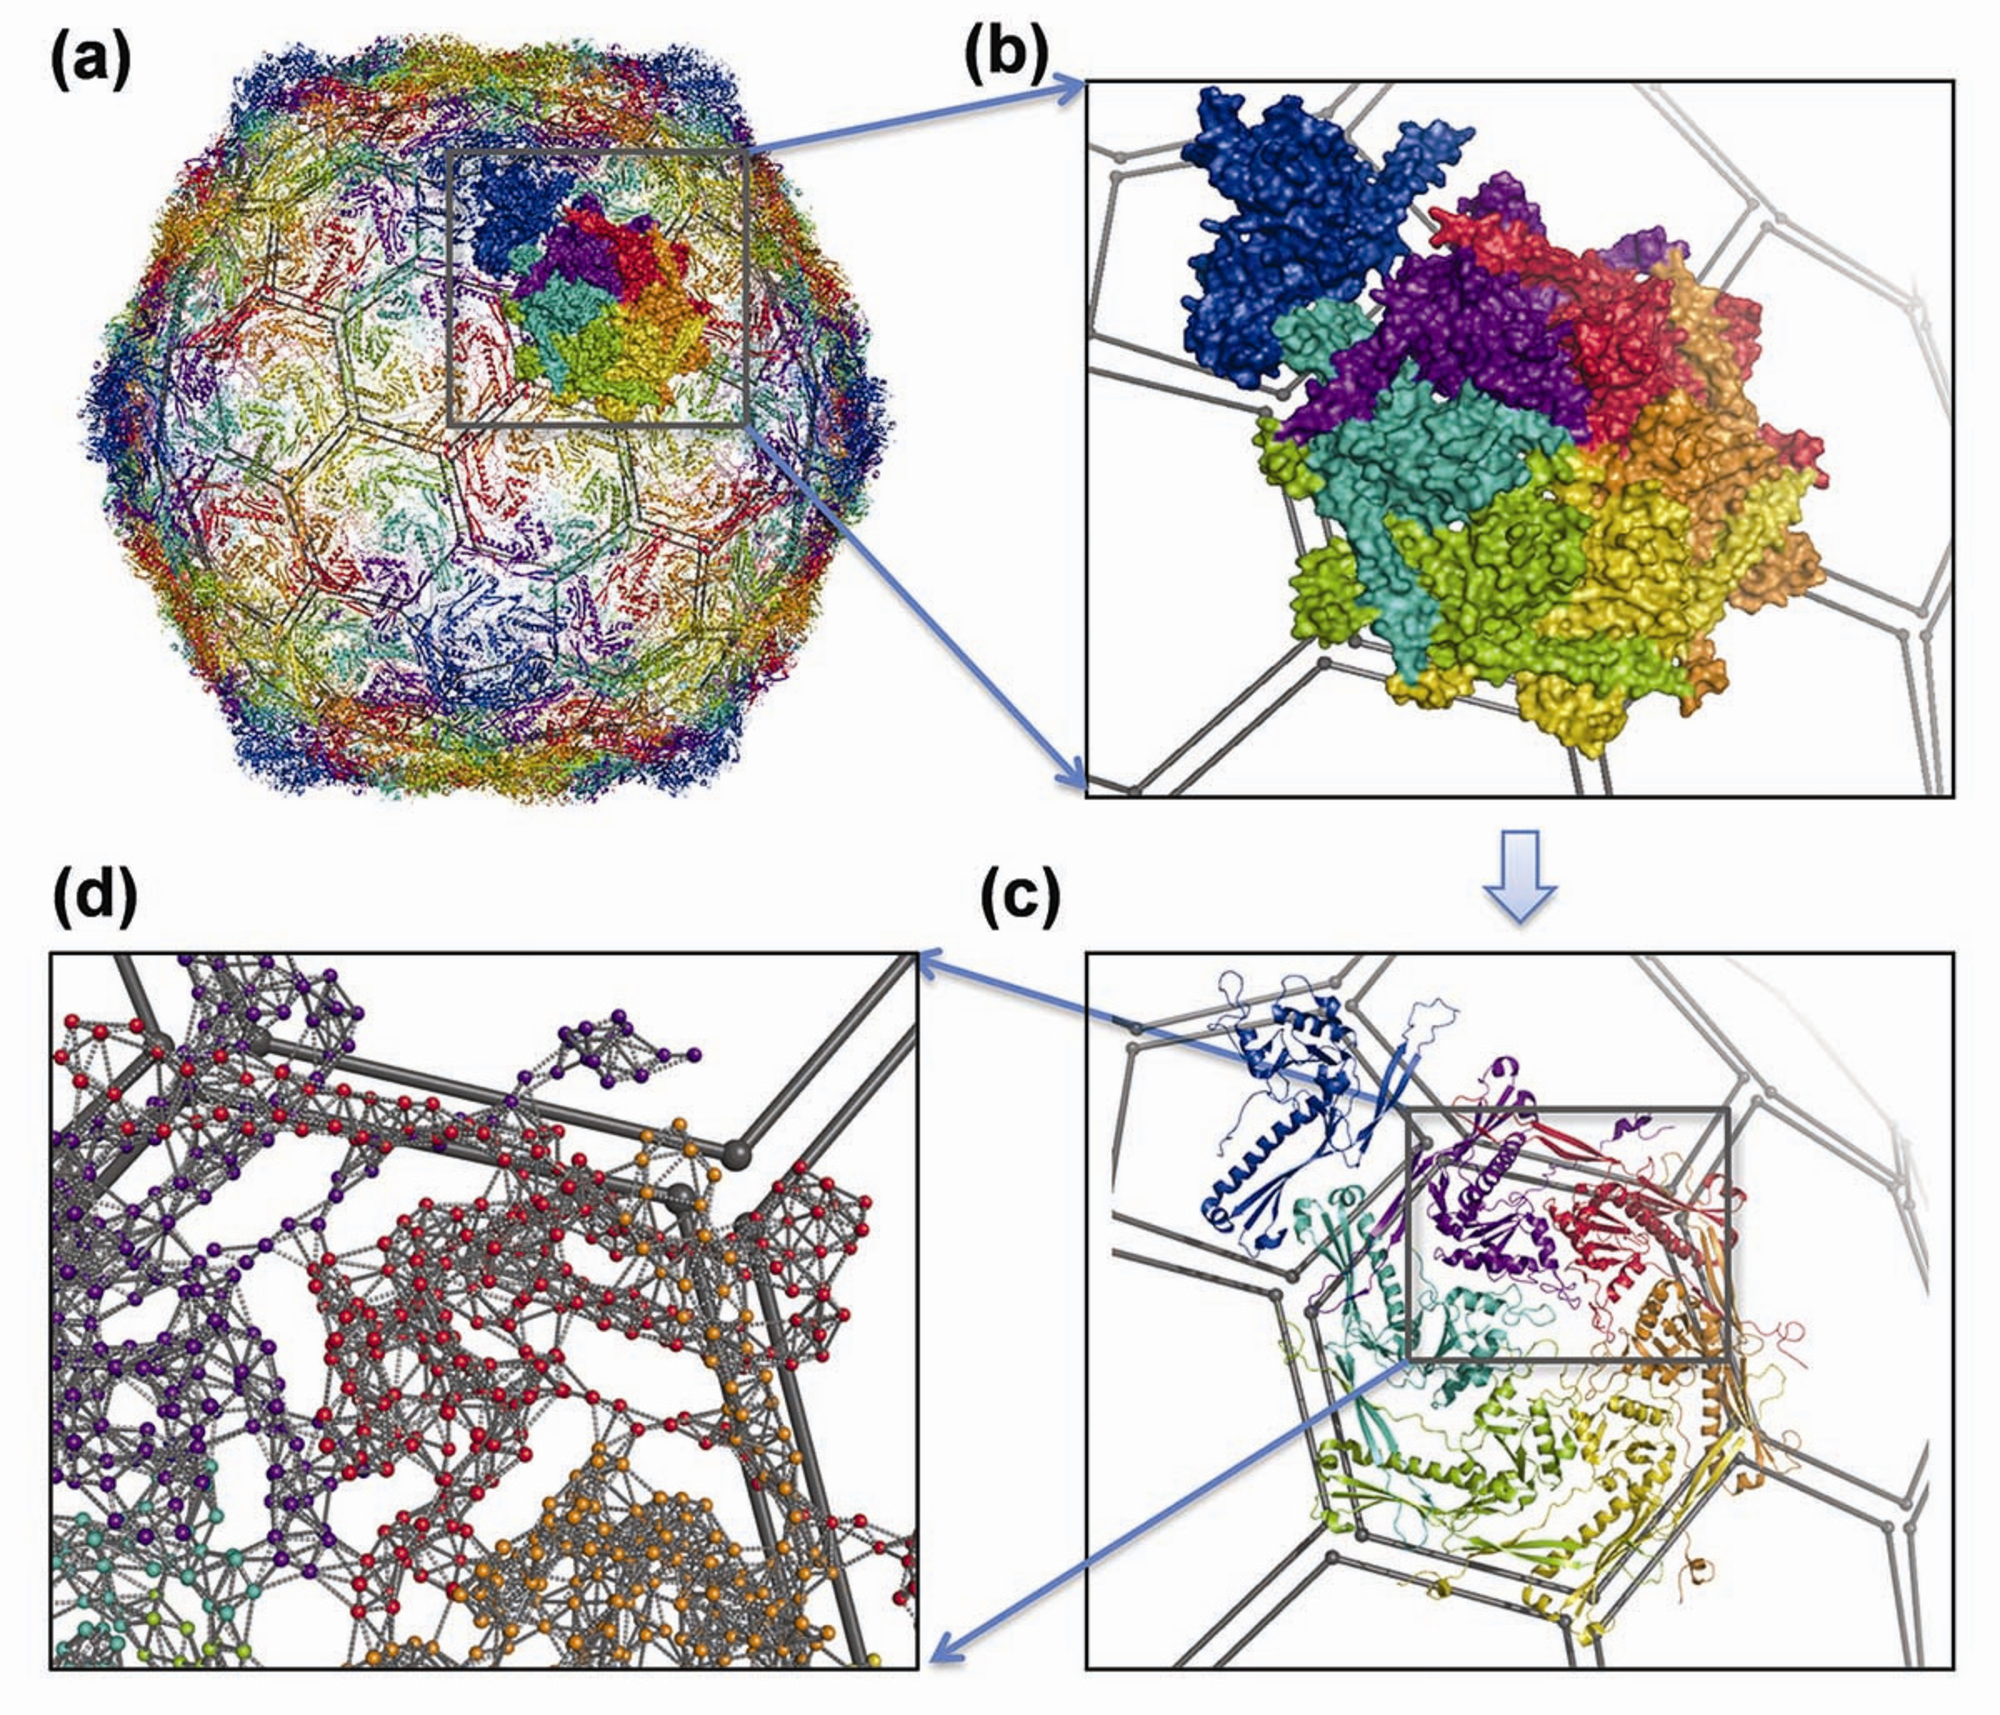
\includegraphics[scale=0.3]{Kap2/dibujo.pdf}%
\caption{ (a) Vista exterior de un c\'{a}pside v\'{i}rico HK97 coloreado por cada cadena, todas las prote\'{i}nas son id\'{e}nticas. (b) Vista del arreglo prote\'{i}nico en una cara del c\'{a}pside. (c) Vista de la estructura secundaria de las prote\'{i}nas (d) Esquema de cada prote\'{i}na mostrando cada uno de sus \'{a}tomos, las aristas de cada cara son carbonos $\alpha$ unidos por lados (ligaduras el\'{a}sticas). Tomado de \cite{Lezon2009ElasticViruses}.} \label{fig:pan}
\end{figure}
\subsubsection{Descripci\'{o}n Mec\'{a}nica del Modelo}

Consid\'{e}rese una biomol\'{e}cula con $N$ part\'{i}culas constituyentes, el tipo de constituyente depende del modelo apropiado para la biomol\'{e}cula, por ejemplo en las prote\'{i}nas como la BPTI, ver \cite{Gur2013GlobalPredictions.}, los constituyentes son los carbonos $\alpha$ de los amino\'{a}cidos.\\

La energ\'{i}a potencial $V$ que representa las interacciones entre los constituyentes de la biomol\'{e}cula, se puede expresar alrededor de las posiciones de equilibrio $\mathbf{q_0}=\mathbf{0}$ tal como describe la teor\'{i}a de peque\~{n}as oscilaciones, ver \cite{Goldstein2001ClassicalMechanics}:
\begin{equation}
V(q)=V(\mathbf{0})+\sum_{i=1}^n\frac{\partial V}{\partial q_i}q_i+\sum_{ij}^{n}\frac{\partial V^2 }{\partial q_i\partial q_j}q_i q_j+...
\end{equation}\label{eq:1}
Donde $q_i$ son los desplazamientos con respecto a las posiciones de equilibrio, $n$ es el n\'{u}mero de posibles desplazamientos en la biomol\'{e}cula. $V(\mathbf{0})$ es el potencial en equilibrio que por conveniencia puede ser calibrado a cero: $V(\mathbf{0})=0$. El hecho de que la energ\'{i}a cin\'{e}tica disminuya hace que los constituyentes vuelvan al estado.\\


El sistema se encuentra alrededor del equilibrio cuando las fuerzas generalizadas se anulan, esto es:
\begin{equation}
\frac{\partial V}{\partial q_i}=0
\end{equation}\label{eq:2}
En este tipo de casos como la energ\'{i}a se minimiza, se dice que hay un equilibrio estable. En un equilibrio estable cuando se hace un incremento de la energ\'{i}a total $E$ se proporciona cierta energ\'{i}a cin\'{e}tica $T_0$ a los constituyentes. Dicha energ\'{i}a  $T_0$  disminuye a medida que el sistema se aleja de la posci\'{o}n de m\'{i}nima energ\'{i}a (la energ\'{i}a potencial aumenta) como se muestra en la figura \ref{fig:pot}. La raz\'{o}n es que $E_0+dE=T+V$, con $E_0+dE$ la energ\'{i}a total del sistema,que se mantiene constante. La explicaci\'{o}n para equilibrios estables e inestables se encuentra en \cite{Goldstein2001ClassicalMechanics}.\\
Considerando la condici\'{o}n del equilibrio \eqref{eq:2} y despreciando desplazamientos de orden superior se tiene que:

\begin{figure}
\centering%
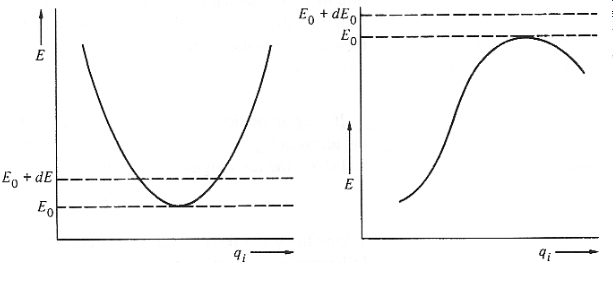
\includegraphics[scale=0.5]{potencial.png}%
\caption{Potencial en funci\'{o}n de la posici\'{o}n} \label{fig:pot}
\end{figure}

\begin{equation}
V(q)=\sum_{ij}^{n}\frac{\partial V^2 }{\partial q_i\partial q_j}q_i q_j
\end{equation}\label{eq:3}
Se identifican las constantes el\'{a}sticas como:
\begin{equation}
k_{ij}=\frac{\partial V^2 }{\partial q_i\partial q_j}
\end{equation}\label{eq:4}

\subsubsection{Ensamble Estad\'{i}stico}
\subsubsection{Modelo de Redes Gaussianas (GNM)}
\subsubsection{Modelos de Resdes Anisotr\'{o}picas (ANM)}
\subsection{An\'{a}lisis de Modos Normales Est\'{a}ndar (NMA)}
Describe un sistema oscilatorio en el que todos los constituyentes del sistema oscilan sinusoidalmente y con la misma frecuencia.
\subsection{An\'{a}lisis por Componentes Principales (PCA)}
\section{Movimientos Locales}
Hace referencia a las simulaciones en las que se incluyen todos los \'{a}tomos junto con las interacciones presentes, es decir, en las que se analizan los \textit{cambios locales}. Estas se pueden simular a un orden de magnitud de los nanosegundos en una m\'{a}quina usual, al respecto ver \cite{Gur2013GlobalPredictions.}.

Como caso particular se pueden tomar los potenciales usados en \cite{Amber2016AmberManual}, que siguen el modelo de Amber. El modelo de Amber tiene en cuenta las contribuciones debidas a:
 \begin{itemize}
\item Interacciones intermoleculares: Son las producidas por los enlaces covalentes entre grupos de \'{a}tomos, las de valencia y las torsiones.
\item Interacciones entre pares: Lennard Jones, electrost\'{a}tico.
\end{itemize}

\subsubsection{An\'{a}lisis por Componentes Principales}

\begin{itemize}
\item 
\end{itemize}
